\documentclass[12pt]{article}
\usepackage{graphicx}
\graphicspath{ {images/} }

\title{Introduction to Chemistry: Reactions and Ratios}




\begin{document}
\maketitle

\section{S1: Atoms and Elements}

Pt gives average masses for each element due to the existence of isotops. 

\begin{itemize}
\item \textbf{Be} Beryllium
\item \textbf{B} Boron
\item \textbf{Ne} Neon
\end{itemize}

\vspace{15mm}

\begin{itemize}
\item \textbf{Protons} determine the identity of an element
\item \textbf{Electrons} determine the charge of the element
\item \textbf{Neutrons} determine the mass of the isotope
\end{itemize}

\section{S2 : The Structure of the Periodic Table}

Group \emph{13} is also called \emph{IIIA}
 

Properties of metals:
\begin{itemize}
\item Malleable (can be shaped)
\item Ductile (drawn into wires)
\item Cations (readily lose electrons)
\item 75\% of the elements are metals
\end{itemize}

Nonmetals readily gain electrons to become anions\\
\\
Metaloids make good semiconductors (e.g. silicon)

Groups 1 \& 2:
\begin{itemize}
\item Alkali metals
\item Alkaline earth metals
\end{itemize}

\section{S3 : Ions and Isotopes}

\begin{equation}
Ion\ charge =\#protons –\#electrons
\end{equation}

Isotopes of Carbon:\\
Carbon-12 (6 neutrons), Carbon-13 (7 neutrons)

\section{S4 : Ionic Bonds}

\begin{itemize}
\item Monatomic anion: change ending to \textbf{-ide}. $S^0->S^{2-}$, Sulfur atom -> Sulfide ion. 
\item Monatomic cations: no change $Na^0->Na^{1+}$, Sodium atom -> Sodium ion.
\end{itemize}

Examples: $Sr^{2+}$ Strontium Ion, $N^{3-}$, Nitride Ion

An electron tries to lower its potential energy.
\begin{itemize}
\item Metal's valence electrons have higher potential elements. 
\item Nonmetals have room for extra electrons and have lower energy levels. 
\end{itemize}

$Na^{1+}F^{1-}$, Ions of Na and Cl stick together due to the electrostatic force. There's no NaCl molecules, only ions.

\section{S4 : Orbital Energy and Ionization Energy Part I}

“Arranged in order of their atomic numbers,
 the elements exhibit \emph{periodicity} in their
 chemical and physical properties."\\
 \\
Periods are \textbf{rows} and groups are \textbf{columns}\\
\\
First ionization energy -- Energy needed to remove an electron from a neutral atom.

\begin{equation}
A + IE = A^+ + e^-
\end{equation}

Metals have \emph{lower} IEs comparing to nonmetals

\begin{figure}[h]
\centering
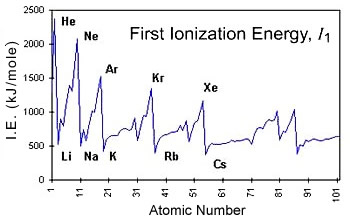
\includegraphics{IEgraph}
\end{figure}


\begin{itemize}
\item For \textbf{like-charged} particles, the energy \textbf{increases} the \textbf{closer} the particles are.
\item For \textbf{oppositely-charged} particles, the energy \textbf{decreases} the \textbf{closer} the particles are. 
\end{itemize}



Coulomb's Law:
\begin{equation}
\delta F = \frac{kq_1q_2}{\epsilon r^2}
\end{equation}

\section {S8 : Intro Stoichiometry Part I}

$HNO_2$ nitrous acid 

\section {S9 : Intro Stoichiometry Part II}

\textbf{Avogadro} constant:
\begin{equation}
6.022*10^{23} = 1\ mole
\end{equation}
The constant defined as the number of atoms in 12 grams of hydrogen of the isotope carbon-12

\end{document}
This is never printed